\section{センサノードグループ化のアプローチ}

% --- トポロジ ---
\subsection{トポロジ}
研究課題4.1のグループ化におけるセンサノード間の通信規格が定められていない課題を解決するため,異種無線によるグループ化を提案する.グループはある数のセンサノードから構成される.グループのトポロジ(図\ref{fig:group_topology}参照)は,グループ内での通信とGLノードとGWノードの通信と2種類あり,ノード間通信の方式は,前者にBLE,後者にLoRaWANを用いる.

\begin{figure}[]
    \begin{center}
    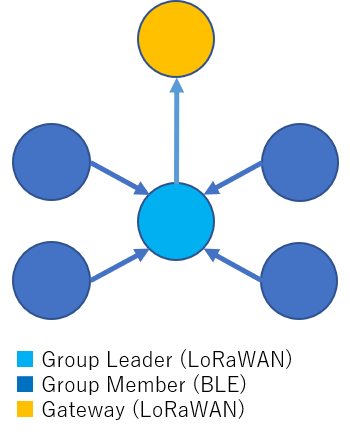
\includegraphics[width=7cm]{figures/v2.0/トポロジ.png}
    \caption{グループ化のトポロジ}
    \label{fig:group_topology}
    \end{center}
\end{figure}

\subsection{グループのスリープ時における通信}
グループ化において,メッセージ集約時以外の通信の振る舞いについて述べる.GMノードは,集約時以外はスリープモードに入り次の通信を待機する.GLノードは,新たなノードが増えた場合にグループに参加するため,BLEにて自身のBLEの固有ID(Perioheral Service UUID)をペイロード(Advertising Channel PDU)に載せ発信する(Advertising).下記にシーケンス(図\ref{fig:group_sleep}参照)を示す.

\begin{figure}[]
    \begin{center}
    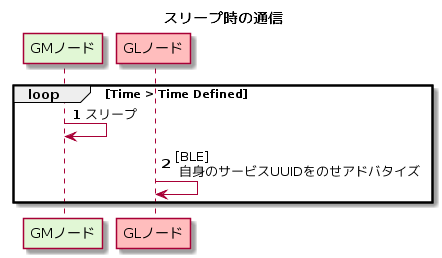
\includegraphics[width=10cm]{figures/v2.0/スリープ時の通信.png}
    \caption{スリープ時のグループ化の通信方式}
    \label{fig:group_sleep}
    \end{center}
\end{figure}

% --- センサネットワーク展開時のグループ化 ---
\subsection{センサネットワーク展開時のグループ化}
研究課題4.2のグループを作成する際に,全てのセンサノードの位置を事前にNSが把握しているというのは現実的ではないという課題を解決するため,センサネットワークが展開される初回起動時にグループを作成する手法を提案する.GWノードがWSNのトポロジを把握しグループを構成するため,各センサノードが初回起動時に周囲のセンサノード情報を探索する.下記にシーケンス(図\ref{fig:group_on_activation}参照)を示す.

\begin{enumerate}
    \item グループを構築するに当たり,GWノードは現在のWSNトポロジを把握する必要がある.そのため,センサノードは起動時にBLEにて自身のLoRaWANの情報(DevEUI)を報知し,同時に周囲のセンサノード情報を収集する(スキャン).センサノードは近傍のセンサノードのリストを作成した後,GWノードへ送信する(図\ref{fig:group_on_activation}シーケンス番号1-2参照).
    \item GWノードは,グループを作成するためセンサノードの情報が到達を一定時間待機する(図\ref{fig:group_on_activation}シーケンス番号3参照).
    \item 収集した情報からグループを作成するため,GWノードはセンサノード情報を一定時間集約した後,センサノードのLoRaWANの固有ID(DevEUI),及び個々のLoRaWAN,BLEの信号強度(RSSi)を用いて重複ノードのないグループを作成し,グループごとに1つGLノードを選出する(図\ref{fig:group_on_activation}シーケンス番号4-5参照).
    \item センサノードがLoRaWANにて次の接続をした際,グループ構成を通知し,各センサノードは,グループの通信に従う(図\ref{fig:group_on_activation}シーケンス番号6-9参照).
\end{enumerate}

\begin{figure}[]
    \begin{center}
    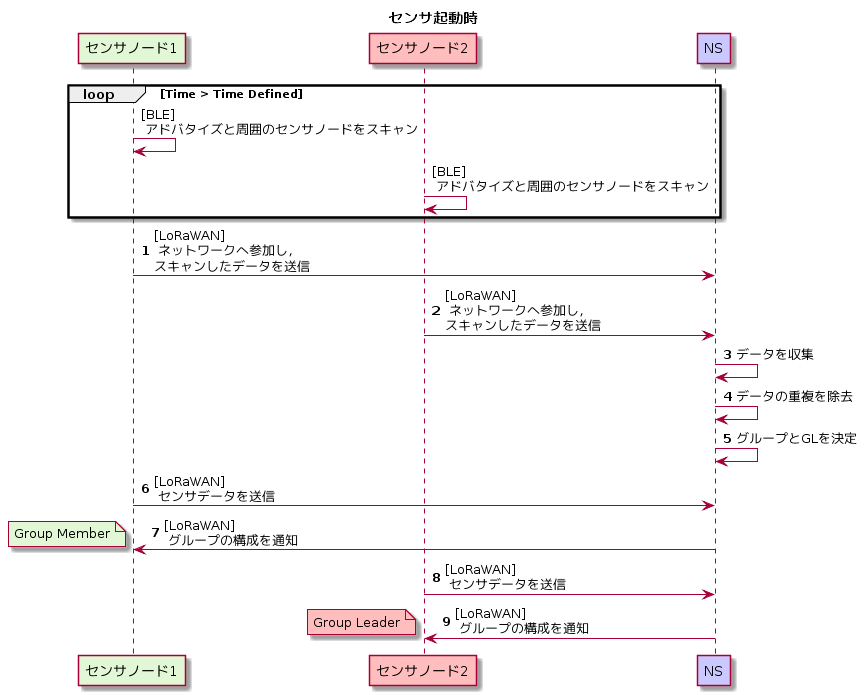
\includegraphics[width=15cm]{figures/v2.0/センサ起動時.png}
    \caption{センサネットワーク展開時のグループ化の通信方式}
    \label{fig:group_on_activation}
    \end{center}
\end{figure}

% --- 定常時のグループ化の通信 ---
\subsection{定常時のグループ化の通信}
定常時のグループの通信フローを述べる.通信方式は,前述したトポロジ(5.2.1参照)に従う.グループ内の通信は,センシングのタイミングが設けられ同期的に通信を行う.下記にシーケンス(図\ref{fig:default_data_flow}参照)を示す.

\begin{enumerate}
    \item GMノードはGLノードとの接続要求のため,BLEにてアドバタイズメントを開始する(図\ref{fig:default_data_flow}シーケンス番号1参照).
    \item GLノードはGMノードとの接続確立のため,BLEにてスキャン要求を開始する(図\ref{fig:default_data_flow}シーケンス番号2参照).
    \item GLノードは,スキャン応答受信後,接続確立する(図\ref{fig:default_data_flow}シーケンス番号3-4参照).
    \item GLノードは,GMノードからセンサデータを集約し,LoRaWANにてGWノードへ送信する(図\ref{fig:default_data_flow}シーケンス番号5-6参照).
\end{enumerate}

\begin{figure}[]
    \begin{center}
    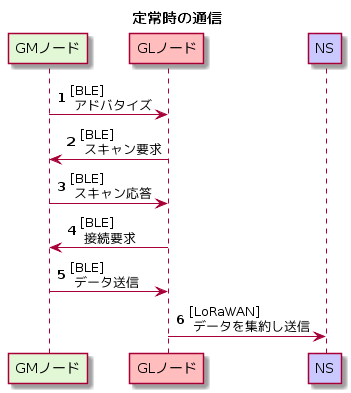
\includegraphics[width=10cm]{figures/v2.0/定常時の通信.png}
    \caption{定常時のグループ化の通信}
    \label{fig:default_data_flow}
    \end{center}
\end{figure}

% --- センサノードの参加・離脱時の振る舞い ---
\subsection{センサノードの参加・離脱時の振る舞い}
研究課題4.2のグループを作成する際に,いくつかのセンサノードの増減が考慮されていない課題を解決するため,グループへ参加・離脱する際の手法を述べる.
前者について下記にシーケンス(図\ref{fig:group_on_join}参照)を示す.

\begin{enumerate}
    \item 前項で述べたスリープ時の通信挙動により,新規センサノードは,起動時にBLEにて周囲の参加可能なグループを探索する.
    \item 参加先を発見した場合は,そのグループに参加する(図\ref{fig:group_on_join}シーケンス2-3番号参照).
    \item そうでない場合はLoRaWANにてセンサデータを送信しGWノードからグループの通知を受ける.グループの参加先がない場合は,LoRaWANにてセンサデータを送信する(図\ref{fig:group_on_join}シーケンス番号2-5参照).
\end{enumerate}

後者について,下記にシーケンス(図\ref{fig:group_on_leave}参照)を示す.

\begin{enumerate}
    \item ノードが停止する(図\ref{fig:group_on_leave}シーケンス1参照).
    \item ノードが故障や電池切れで離脱する場合は,GLノードがデータが欠損した状態で送信する(図\ref{fig:group_on_leave}シーケンス2-3参照).
    \item NSがデバイスを管理しているので,一定期間,センサデータがGWノードに届かなかった際に,グループリストからセンサノードを取り除く(図\ref{fig:group_on_leave}シーケンス4参照).
    \item GLノードの次回通信時に,更新したグループリストを通知する(図\ref{fig:group_on_leave}シーケンス5参照).
\end{enumerate}

\begin{figure}[]
    \begin{center}
    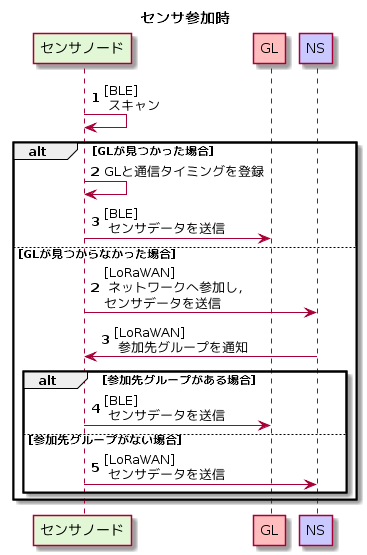
\includegraphics[width=10cm]{figures/v2.0/センサ参加時.png}
    \caption{ネットワーク参加時の振る舞い}
    \label{fig:group_on_join}
    \end{center}
\end{figure}


\begin{figure}[]
    \begin{center}
        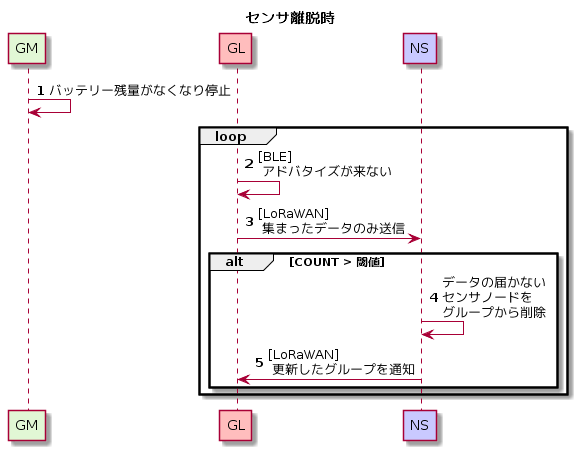
\includegraphics[width=13cm]{figures/v2.0/センサ離脱時.png}
    \caption{ネットワーク離脱時の振る舞い}
    \label{fig:group_on_leave}
    \end{center}
\end{figure}